%% Copernicus Publications Manuscript Preparation Template for LaTeX Submissions
%% ---------------------------------
%% This template should be used for copernicus.cls
%% The class file and some style files are bundled in the Copernicus Latex Package, which can be downloaded from the different journal webpages.
%% For further assistance please contact Copernicus Publications at: production@copernicus.org
%% https://publications.copernicus.org/for_authors/manuscript_preparation.html

%% copernicus_rticles_template (flag for rticles template detection - do not remove!)

%% Please use the following documentclass and journal abbreviations for discussion papers and final revised papers.

%% 2-column papers and discussion papers
\documentclass[, manuscript]{copernicus}



%% Journal abbreviations (please use the same for preprints and final revised papers)

% Advances in Geosciences (adgeo)
% Advances in Radio Science (ars)
% Advances in Science and Research (asr)
% Advances in Statistical Climatology, Meteorology and Oceanography (ascmo)
% Annales Geophysicae (angeo)
% Archives Animal Breeding (aab)
% Atmospheric Chemistry and Physics (acp)
% Atmospheric Measurement Techniques (amt)
% Biogeosciences (bg)
% Climate of the Past (cp)
% DEUQUA Special Publications (deuquasp)
% Drinking Water Engineering and Science (dwes)
% Earth Surface Dynamics (esurf)
% Earth System Dynamics (esd)
% Earth System Science Data (essd)
% E&G Quaternary Science Journal (egqsj)
% EGUsphere (egusphere) | This is only for EGUsphere preprints submitted without relation to an EGU journal.
% European Journal of Mineralogy (ejm)
% Fossil Record (fr)
% Geochronology (gchron)
% Geographica Helvetica (gh)
% Geoscience Communication (gc)
% Geoscientific Instrumentation, Methods and Data Systems (gi)
% Geoscientific Model Development (gmd)
% History of Geo- and Space Sciences (hgss)
% Hydrology and Earth System Sciences (hess)
% Journal of Bone and Joint Infection (jbji)
% Journal of Micropalaeontology (jm)
% Journal of Sensors and Sensor Systems (jsss)
% Magnetic Resonance (mr)
% Mechanical Sciences (ms)
% Natural Hazards and Earth System Sciences (nhess)
% Nonlinear Processes in Geophysics (npg)
% Ocean Science (os)
% Polarforschung - Journal of the German Society for Polar Research (polf)
% Primate Biology (pb)
% Proceedings of the International Association of Hydrological Sciences (piahs)
% Safety of Nuclear Waste Disposal (sand)
% Scientific Drilling (sd)
% SOIL (soil)
% Solid Earth (se)
% The Cryosphere (tc)
% Weather and Climate Dynamics (wcd)
% Web Ecology (we)
% Wind Energy Science (wes)

% Pandoc citation processing

% The "Technical instructions for LaTex" by Copernicus require _not_ to insert any additional packages.
% 
% tightlist command for lists without linebreak
\providecommand{\tightlist}{%
  \setlength{\itemsep}{0pt}\setlength{\parskip}{0pt}}


%%\usepackage{booktabs}
\usepackage{longtable}
\usepackage{array}
\usepackage{multirow}
\usepackage{wrapfig}
\usepackage{float}
\usepackage{colortbl}
\usepackage{pdflscape}
\usepackage{tabu}
\usepackage{threeparttable}
\usepackage{threeparttablex}
\usepackage[normalem]{ulem}
\usepackage{makecell}
\usepackage{xcolor}
%
\begin{document}


\title{Informing forest carbon inventories under the Paris Agreement
using the Global Forest Carbon Database (ForC v4.0)}


\Author[1,2 *]{Kristina J.}{Anderson-Teixeira}
\Author[1]{Valentine}{Herrmann}
\Author[1]{Madison}{Williams}
\Author[1]{Teagan}{Rogers}
\Author[1,3]{Rebecca}{Banbury Morgan}
\Author[4]{Ben}{Bond-Lamberty}
\Author[5]{Susan}{Cook-Patton}


\affil[1]{Center for Conservation Ecology, Smithsonian's National Zoo \&
Conservation Biology Institute, Front Royal, VA, United States}
\affil[2]{Forest Global Earth Observatory, Smithsonian Tropical Research
Institute, Panama, Republic of Panama}
\affil[3]{School of Geography, University of Leeds, Leeds, UK}
\affil[4]{Joint Global Change Research Institute, Pacific Northwest
National Laboratory, College Park, MD, United States}
\affil[5]{The Nature Conservancy; Arlington VA 22203, USA}

\runningtitle{Informing forest CO\textsubscript{2} inventories with
ForC}

\runningauthor{Anderson-Teixeira et al.}


\correspondence{Kristina J.\ Anderson-Teixeira\ (teixeirak@si.edu)}



\received{}
\pubdiscuss{} %% only important for two-stage journals
\revised{}
\accepted{}
\published{}

%% These dates will be inserted by Copernicus Publications during the typesetting process.


\firstpage{1}

\maketitle






\begin{center}\rule{0.5\linewidth}{0.5pt}\end{center}

\emph{THIS IS AN IN-PREP MANUSCRIPT.}

\begin{center}\rule{0.5\linewidth}{0.5pt}\end{center}

\textbf{Abstract.} Forests are critical for climate change mitigation
and constitute a substantial portion of planned net emissions reductions
under the 2015 Paris Agreement. However, the efficacy of greenhouse gas
mitigation planning and reporting is dependent upon the quality of
available emission factors data, including forest carbon (C) stocks and
changes therein. Tens of thousands of relevant forest C estimates have
been published, yet are not readily accessible to the practitioners
compiling national greenhouse gas inventories. Many of these data have,
however, been compiled in the Global Forest C database (ForC;
https://forc-db.github.io/) and stand to be of value to greenhouse gas
inventories if made available through the Emission Factor Database
(EFDB) of the International Panel on Climate Change (IPCC). Here, we
develop and document a process for semi-automated submission of data
from ForC into the EFDB, assess the data available and submitted to
date, and provide recommendations for improving forest data collection,
analysis, and reporting to improve inventories of forest-sector
greenhouse gas emissions and removals. We begin by reconciling
terminology and mapping ForC fields into EFDB. This process required
some updates to the ForC database structure, leading to the release of a
new version of ForC (v4.0; described here). As of June 09, 2023, ForC
contained \textasciitilde19316 independent records relevant to EFDB,
1438 of which have been submitted to date. Among the data in ForC, there
is disproportionate representation of biomass (particularly aboveground)
stocks, with far fewer records for dead organic matter and soil C, and
relatively few or no records for net annual increments or C fluxes into
(gains) or out of (losses) the IPCC-defined C pools. Geographic
representation is also quite uneven, with the highest densities of
relevant records in temperate forests, and with relatively scant
representation of tropical forests in Africa and Asia. In the future,
forest C estimates in EFDB can be improved through targeted research to
fill critical gaps, reporting of information required by IPCC, and
continued submission of data from scientific publications to the EFDB.
Given that climate change is rapidly impacting the world's forests,
timely reporting of recent estimates will be especially critical to
accurate forest C inventories.

\introduction[Introduction]

Forests are critical to management of the atmospheric concentration of
the greenhouse gas carbon dioxide (CO\textsubscript{2}), and thereby
climate change. In recent decades, CO\textsubscript{2} uptake by
forests, woodlands, and savannas has exceeded releases from
deforestation and other severe disturbances, resulting in a net carbon
CO\textsubscript{2} sink of \textasciitilde0.88 Gt C
yr\textsuperscript{-1} \citep[all biomes with trees,][]{xu_changes_2021}
to \textasciitilde1.6 Gt C yr\textsuperscript{-1} \citep[forests
only,][]{harris_global_2021}. This has offset an estimated 10\% to 18\%
of anthropogenic CO\textsubscript{2} emissions from fossil fuels and
cement \citep{xu_changes_2021, harris_global_2021}, dramatically slowing
the pace of atmospheric CO\textsubscript{2} accumulation and associated
climate change. The future of this important CO\textsubscript{2} sink is
highly uncertain, and depends upon both forest responses to climate
change, which are likely to reduce the sink strength
\citep{mcdowell_pervasive_2020, hammond_global_2022}, and human
conservation, restoration, and management of forests
\citep{ipcc_climate_2019, ipcc_climate_2022}.

Forests play a substantial role in international plans for climate
change mitigation under the Paris Agreement
\citep{unfccc_adoption_2015}. Forest conservation, reforestation, and
improved sustainable management all have significant -- and relatively
cost-effective -- potential as climate change mitigation options, with
conservation and reforestation having the fourth and fifth largest net
emission reduction potentials or all mitigation options
\citep{ipcc_summary_2022}. As of 2016, forest-based mitigation accounted
for 26\% of total planned greenhouse gas mitigation within Nationally
Determined Contributions under the Paris Agreement
\citep{grassi_key_2017}. Yet, envisioned forest-based climate change
mitigation initiatives do not always correspond to actual emission
reductions through on-the-ground implementation
\citep[e.g.,][]{badgley_systematic_2022}. One critical need for ensuring
that forest-based climate change mitigation initiatives are effective is
realistic planning and reporting, underlain by solid scientific data
\citep{anderson-teixeira_effective_2022, deng_comparing_2021}.

The International Panel on Climate Change (IPCC) provides guidance for
national greenhouse gas inventories for reporting to the United Nations
Framework Convention on Climate Change
\citep[UNFCCC,][]{ipcc_2006_2006, ipcc_2019_2019}. Under this guidance,
greenhouse gas inventories include all managed land, including most of
the world's forest land \citep{ogle_delineating_2018}. The IPCC
inventory guidelines include specific instructions for inventories for
greenhouse gas (mainly CO\textsubscript{2}) exchanges between forest
land and the atmosphere \citep{ipcc_agriculture_2006, ipcc_2019_2019}. A
tiered approach is employed, where the lowest tier (Tier 1) represents
the simplest approach and relies on default parameter values -- for
example, forest carbon (C) stocks values by ecozone
\citep{fao_global_2012} and forest age class derived as the average of
published estimates \citep{ipcc_2019_2019, rozendaal_aboveground_2022}.
Tier 1 values have improved over the years as more of the relevant
underlying data has become available
\citep{requenasuarez_estimating_2019, rozendaal_aboveground_2022}, but
there remains room for improvement as datasets grow and become more
widely accessible. For example, the year following the release of the
latest IPCC guidelines, a more thorough analysis of C accumulation in
regrowth forests found that IPCC's Tier 1 default values underestimated
C sequestration by 32\% on average and failed to capture eight-fold
variation within ecozones \citep{cook-patton_mapping_2020}. In addition,
it was revealed that C stocks in mature African tropical montane forests
were two-thirds higher than the IPCC Tier 1 values for these forests
\citep{cuni-sanchez_high_2021}. This rapid evolution of scientific
information on C cycling in forests is valuable for informing climate
change mitigation efforts but requires improved mechanisms for
communicating the latest information from scientific researchers to the
practitioners who need reliable estimates for greenhouse gas mitigation
planning. Moreover, high variability of forest C cycling within ecozones
\citep[e.g.,][]{cook-patton_mapping_2020, cuni-sanchez_high_2021}
implies that it is useful for practitioners to have access to
locally-specific information, when available.

To improve data accessibility for preparing greenhouse gas estimates,
the IPCC created the Emission Factor Database (EFDB;
\url{https://www.ipcc-nggip.iges.or.jp/EFDB/main.php}), which is
intended as a recognized library of emission factors and other
parameters that can be used for estimating greenhouse gas emissions and
removals. The EFDB can be used both for efforts to tally a nation's
intended or accomplished greenhouse gas reductions, or as a basis of
comparison for external parties to evaluate these inventories. The EFDB
encourages researchers to submit estimates of emission factors or other
related parameters from peer-reviewed journal papers or other accepted
sources for inclusion in the database. In the case of forests, emission
factors include C stocks, net annual increments, and annual fluxes for
various pools \citep{ipcc_2006_2006, ipcc_2019_2019}.

The Global Forest Carbon Database, ForC
(\url{https://forc-db.github.io/}), is the largest collection of
published estimates of forest C stocks, increments, and annual fluxes
\citep{anderson-teixeira_forc_2018, anderson-teixeira_carbon_2021}. ForC
includes data ingested from individual publications and relevant
databases, including the Global Reforestation Opportunity Assessment
(GROA) database \citep[database doi:
10.5281/zenodo.3983644]{cook-patton_mapping_2020}, and the global soil
respiration database
\citep[SRDB-V5,][]{bond-lamberty_global_2010, jian_restructured_2021}.
As of June 09, 2023, ForC contained 39848 records from 10589 plots in
1535 distinct geographical areas, along with records of stand age and
disturbance history. As such, ForC is positioned to improve
forest-related estimates of CO\textsubscript{2} emissions and removals
through the submission of data to the EFDB. The purpose of this
publication is to document that process and provide recommendations for
future improvements.

Here, we (1) review IPCC methods and definitions applied to estimate
CO\textsubscript{2} emissions and removals from forest in the context of
typical forest C estimation methodologies; (2) describe mapping of ForC
to IPCC's EFDB; (3) describe updates to ForC (ForC v4.0), most of which
were implemented to facilitate data submission to EFDB; (4) summarize
the data in ForC relevant to EFDB and records that have been submitted
to date; and (5) provide recommendations as to how the scientific
community can better provide useful data for forest C inventories under
the Paris Agreement.

\section{IPCC methods and definitions}

The end goal of IPCC greenhouse gas inventories is to quantify
greenhouse gas emissions to, or withdrawals from, the atmosphere on an
annual basis, most commonly on a national level
\citep{ipcc_2006_2006, ipcc_2019_2019}. For each stratum of subdivision
within a land-use category, annual stock changes (\(\Delta C\); t C
yr\textsuperscript{-1}) are calculated as the sum of changes in various
pools (described in section 2.1), plus any harvested wood products. For
each pool, \(\Delta C\) may be calculated using the ``Gain-Loss
Method'', which takes the difference between gains and losses, or using
the ``Stock-Difference Method'', which computes \(\Delta C\) based on C
stocks at two points in time \citep{ipcc_2006_2006}. Thus, C cycle
variables relevant to the IPCC methodology and to EFDB include C stocks,
net annual increments, and fluxes in the IPCC-defined pools.

\subsection{Carbon pools}

Forest ecosystem C pools may be parsed in various ways, and while
certain definitions and thresholds are more common than others, there is
no single standard for measuring or reporting that is adhered to by all
-- or even most -- scientific studies. IPCC parses forest C pools into
biomass (aboveground and belowground), dead organic matter (dead wood
and litter), and soil organic matter (Table 1). While there is some
flexibility around the components included in each pool, each national
inventory must apply these in a consistent manner.

\begin{table}

\caption{\label{tab:table_pools}\textbf{IPCC-defined forest carbon pools with definitions and measurement methods.} Definitions from IPCC Table 1.1. (See Table 1.1 in IPCC guidance).}
\centering
\begin{tabu} to \linewidth {>{\raggedright}X>{\raggedright}X>{\raggedright}X>{\raggedright}X}
\hline
\textbf{pool} & \textbf{definition} & \textbf{important sources of estimate variation} & \textbf{IPCC guidance}\\
\hline
aboveground biomass & all biomass of living vegetation & minimum size censused & may exclude understory if minor component\\
\hline
 &  & include non-dicot trees? & yes\\
\hline
 &  & include dead standing? & no\\
\hline
 &  & biomass allometry & Tier 1 defaults draw on a variety of allometric models\\
\hline
belowground biomass & all biomass of live roots & all factors relevant to aboveground biomass & see above\\
\hline
 &  & allometry or assumed ratio of below- to above-ground biomass (R) & can estimate based on R\\
\hline
 &  & minimum root diameter & may exclude fine roots; suggested diameter cutoff of 2 mm for fine roots\\
\hline
dead wood & all non-living woody biomass above a specified diameter, aboveground or belowground & minimum diameter & 10 cm default, but may be chosen by country\\
\hline
 &  & include belowground? & \vphantom{1} yes\\
\hline
litter & all non-living biomass smaller than dead wood but larger than soil organic matter, in various states of decomposition both above or within the mineral or organic soil & maximum diameter (= minimum diameter for deadwood) & 10 cm default, but may be chosen by country\\
\hline
 &  & minimum size (= size limit for soil organic matter) & suggested 2 mm\\
\hline
 &  & layers included & entire O horizon: litter (OL),  fumic (OF),  and  humic (OH) layers\\
\hline
 &  & include belowground? & yes\\
\hline
soil organic matter & organic carbon in mineral soils to a specified depth & sampling depth & 30 cm default, but may be chosen by country\\
\hline
\end{tabu}
\end{table}

\subsubsection{Biomass}

Biomass includes living vegetation, above- and below-ground, both woody
and herbaceous, but with a focus on woody plants and trees given their
much greater potential to sequester large amounts of C
\citep{ipcc_2006_2006}.

Aboveground biomass, which is typically \textless200 t C
ha\textsuperscript{-1} but can exceed 700 t C ha\textsuperscript{-1}
\citep{anderson-teixeira_carbon_2021}, is defined by the IPCC as ``all
biomass of living vegetation above the soil including stems, stumps,
branches, bark, seeds, and foliage''
\citep{ipcc_good_2003, ipcc_2006_2006}. IPCC's guidance is that the
understory may be excluded the understory if it constitutes a ``minor''
component \citep[defined as \textless{} 25 - 30 \% of emissions/removals
for the overall category,][]{ipcc_2006_2006}, and where a commonly
applied minimum size sampling threshold for mature forests would be 10
cm stem diameter at breast height (DBH). A recent study characterizing
the contributions of trees in different DBH classes to ecosystem C
stocks and fluxes found that trees 1 - 10 cm DBH contributed up to
\textasciitilde8\% aboveground biomass, \textasciitilde17\% aboveground
woody net primary productivity (\(ANPP_{woody.stem}\)), and
\textasciitilde20\% woody mortality (\(M_{woody}\)) of mature
closed-canopy forests worldwide \citep{piponiot_distribution_2022}, and
therefore stems \textless{} 10 cm DBH can usually be considered a minor
component of aboveground biomass for these forests. In regrowth forests,
woodlands, or savannas, small trees and shrubs contribute a much larger
proportion of C stocks and fluxes
\citep{lutz_global_2018, piponiot_distribution_2022, hughes_biomass_1999},
and, correspondingly, biomass estimates for these ecosystems tend
include smaller size classes. While IPCC guidance specifies that all
living vegetation should be included in biomass estimates, forest
censuses and biomass estimates do not consistently include life forms
other than dicot trees (e.g., lianas, ferns, palms, bamboo), although
these do tend to be censused when they constitute a large proportion of
the biomass \citep[e.g.,][]{fukushima_recovery_2007}. Further, it is
important to note that the IPCC definition of aboveground biomass
excludes standing dead wood, which is included in remote sensing biomass
estimates \citep{duncanson_aboveground_2021}.

A universal challenge in estimating biomass (living or dead) from forest
census data is applying appropriate allometric models to convert DBH
measurements to biomass, and such selection has an enormous influence on
estimates of biomass stocks, increments, and fluxes
\citep{clark_landscapescale_2000, clark_net_2001}. While trusted and
standardized allometric models are becoming increasingly available
\citep{chave_improved_2014, rejou-mechain_biomass_2017, gonzalez-akre_allodb_2022},
large uncertainties remain. IPCC Tier 1 values currently draw on studies
applying a variety of allometric models
\citep[e.g.,][]{requenasuarez_estimating_2019, rozendaal_aboveground_2022}.

Belowground biomass is defined as ``all biomass of live roots''
\citep{ipcc_good_2003, ipcc_2006_2006}, a definition including both
coarse roots, whose biomass is typically estimated based on stem
censuses and allometries or belowground to aboveground biomass ratios,
and fine roots, whose biomass is typically estimated via extraction of
roots from soil samples. The former, which is typically \textless40 t C
ha\textsuperscript{-1} \citep{anderson-teixeira_carbon_2021}, is
methodologically linked to aboveground biomass estimates, sharing the
same methodological sources of variation, and tending to be very
uncertain \citep[e.g.,][]{keller_biomass_2001}. Fine root biomass
generally constitutes a much smaller C pool \citep[typically \textless5
t C ha\textsuperscript{-1},][]{anderson-teixeira_carbon_2021}, and IPCC
guidance is that it can be excluded when fine roots cannot be
distinguished empirically from soil organic matter or litter
\citep{ipcc_2006_2006}, which can be a painstaking process. Field
methods for estimating root biomass are highly variable
\citep{freschet_starting_2021}. IPCC's default method for Tier 1
estimates is to apply a ratio of belowground to aboveground biomass,
with default factors defined based on ecological zone, continent, and
forest age \citep{ipcc_2006_2006, ipcc_2019_2019}.

\subsubsection{Dead Organic Matter}

Dead organic matter includes all non-living biomass that is not within
the mineral soil layer and smaller than the litter size threshold. Its
inclusion in inventories is not required under Tier 1 methodology for
Forest Land remaining Forest Land (see section 2.2), but is required for
land that has transitioned to or from forest within the past 20 years
\citep{ipcc_2006_2006}.

Dead wood, which is typically \textless50 t C ha\textsuperscript{-1} but
can exceed 150 t C ha\textsuperscript{-1}
\citep{anderson-teixeira_carbon_2021}, is defined by IPCC as ``all
non-living woody biomass not contained in the litter, either standing,
lying on the ground, or in the soil''
\citep{ipcc_good_2003, ipcc_2006_2006}. This pool includes standing and
fallen dead wood, stumps, and dead roots of diameter ≥10 cm (or a
diameter specified by the country). Dead wood stocks and fluxes can be
quite variable across forests \citep{anderson-teixeira_carbon_2021}, and
can at times be the dominant pool in a forest ecosystem \citep[e.g.,
following a severe natural disturbance,][]{carmona_coarse_2002}.
However, aboveground dead wood remains relatively poorly characterized
at a global scale \citep{anderson-teixeira_carbon_2021}, and belowground
dead wood is rarely studied \citep{merganicova_dadwood_2012}. In turn,
dead wood pools are poorly characterized in large-scale forest C budgets
\citep{pan_large_2011, harris_global_2021}, and IPCC's latest Tier 1
default values are based on just 1-31 references per climate zone
\citep[Table 2.2 in][]{ipcc_2019_2019}.

Litter, which is typically \textless40 t C ha\textsuperscript{-1} but
can exceed 100 t C ha\textsuperscript{-1}
\citep{anderson-teixeira_carbon_2021}, is defined by IPCC as including
``all non-living biomass with a diameter less than a minimum diameter
chosen by the country (for example 10 cm), lying dead, in various states
of decomposition above the mineral or organic soil''
\citep{ipcc_good_2003, ipcc_2006_2006}. As noted above, live fine roots
may be included in litter when difficult to separate empirically. The
definition includes the entire O horizion, including litter (OL), fumic
(OF), and humic (OH) layers, in addition to litter embedded within the
soil. This definition contrasts with empirical studies that focus on
aboveground litter, often including only the OL layer in the definition
of litter, and do not always specify the components included. Similar to
dead wood, litter is poorly characterized in large-scale forest C
budgets \citep{pan_large_2011, harris_global_2021}, and IPCC's latest
Tier 1 default values are based on just 1-7 references per climate zone
\citep[Table 2.2 in][]{ipcc_2019_2019}.

\subsubsection{Soil Organic Matter/ Carbon}

Soil organic matter/ carbon (SOM/ SOC), which is typically
\textgreater100 t C and can exceed 300 t C in the top two meters of soil
\citep{sanderman_soil_2017}, is defined by IPCC as ``organic carbon in
mineral and organic soils (including peat) to a specified depth chosen
by the country and applied consistently through the time series''
\citep{ipcc_good_2003, ipcc_2006_2006}. Live fine roots may be included
with soil organic matter when it is not feasible to distinguish them
empirically. The greatest source of methodological variation in
measuring SOM/ SOC is sampling depth, which has a suggested default of
30 cm but may vary by country provided that consistent criteria are
applied.

\subsection{Land classification}

IPCC defines land-use categories to include six categories -- Forest
Land, Grassland, Wetlands, Cropland, Settlements, and Other Land
\citep{ipcc_2006_2006}. Sub-divisions include land that has remained in
a particular category for \textgreater20 years (e.g., Forest Land
remaining Forest Land) and land that has been converted from one
category to another in the past 20 years (e.g., Cropland converted to
Forest Land). Forest Land is defined as at least 10-30\% crown cover of
trees with potential to reach a minimum height of 2-5 m \emph{in situ},
and shorter-stature natural vegetation would be classified as Grassland
\citep{ipcc_good_2003}. Definitions of forest are allowed to vary by
country, but must be applied consistently. Forest Land includes land
where vegetation temporarily falls below the threshold values for forest
(e.g., due to disturbance), but is expected to exceed those thresholds
in the future \citep{ipcc_good_2003}.

The UNFCCC requires greenhouse gas reporting for all managed lands in a
country, where management is defined as ``human interventions and
practices have been applied to perform production, ecological or social
functions'' \citep{ipcc_2006_2006}. This expansive definition of managed
land implies that the majority of Forest Land in most countries is
managed. However, the definition is applied differently across
countries, and the majority of governments have yet to report their
approach for defining managed land or provide maps of managed land
\citep{ogle_delineating_2018, deng_comparing_2021}.

\section{Updates to ForC (ForC v4.0)}

This section describes changes relative to ForC v3.0
\citep{anderson-teixeira_carbon_2021}. Previous versions of ForC
\citep{anderson-teixeira_carbon_2016, anderson-teixeira_forc_2018, anderson-teixeira_carbon_2021}
contained most of the information required by EFDB, and, more broadly,
to inform C stock change calculations under the Paris Agreement.
However, modest changes to the structure and contents of ForC were
needed in order to provide all information required by EFDB and to
improve ForC's capacity to serve as a repository of valuable information
for forest C inventories under IPCC guidelines. To support export of
data to EFDB, and to improve the overall quality of the ForC database,
we added or modified 18 fields (Appendix A), defined 15 new variables,
implemented enhanced quality control, manually reviewed \textgreater1963
records to obtain additional required information, and added 329 new
records.

\subsection{New or modified fields}

We added or modified a total of 18 fields (Appendix A). Most notably,
these included improvement of the representation of uncertainty,
recording of original units and organic matter to C conversion factors,
and expanding the information recorded in the citations table. For the
latter, we used an R script to automatically harvest (scrape) the URL,
citation, abstract and language of the publications, based on their DOI,
using R package \texttt{rvest}\citep{wickham_rvest_2022}. That
information was manually retrieved when the web scraping failed.

\subsection{New variables}

To create structure for EFDB-relevant records, we added a total of 15
new variables to the set of named and defined variables (Fig. 1),
counting each pair of variables with units in C (ending in \texttt{\_C})
or organic matter (ending in \texttt{\_OM}) as one. The majority of
these were increment variables (n=11), adding to only one previously
defined increment variable (aboveground biomass increment,
\emph{delta.agb}). These are directly related to C stocks as previously
defined in ForC, with ``\emph{delta.}'' added in front of the variable
name. Further, we added variables capturing the belowground component of
woody mortality (\emph{woody.mortality\_root}) and the combined
aboveground and belowground components of woody mortality
(\emph{woody.mortality}). Although most of these variables lacked
records in ForC as of June 09, 2023, their addition gave the structure
such that records can be populated over time. Finally, to provide better
definition of the previously existing variable \emph{organic.layer},
which has a nebulous definition that reflects the varied definitions
adopted by original studies, we added two clearly defined variables:
\emph{litter} (relatively undecomposed plant material/ OL horizon), and
\emph{O.horizon} (entire O-horizon, including OL).

\begin{figure}
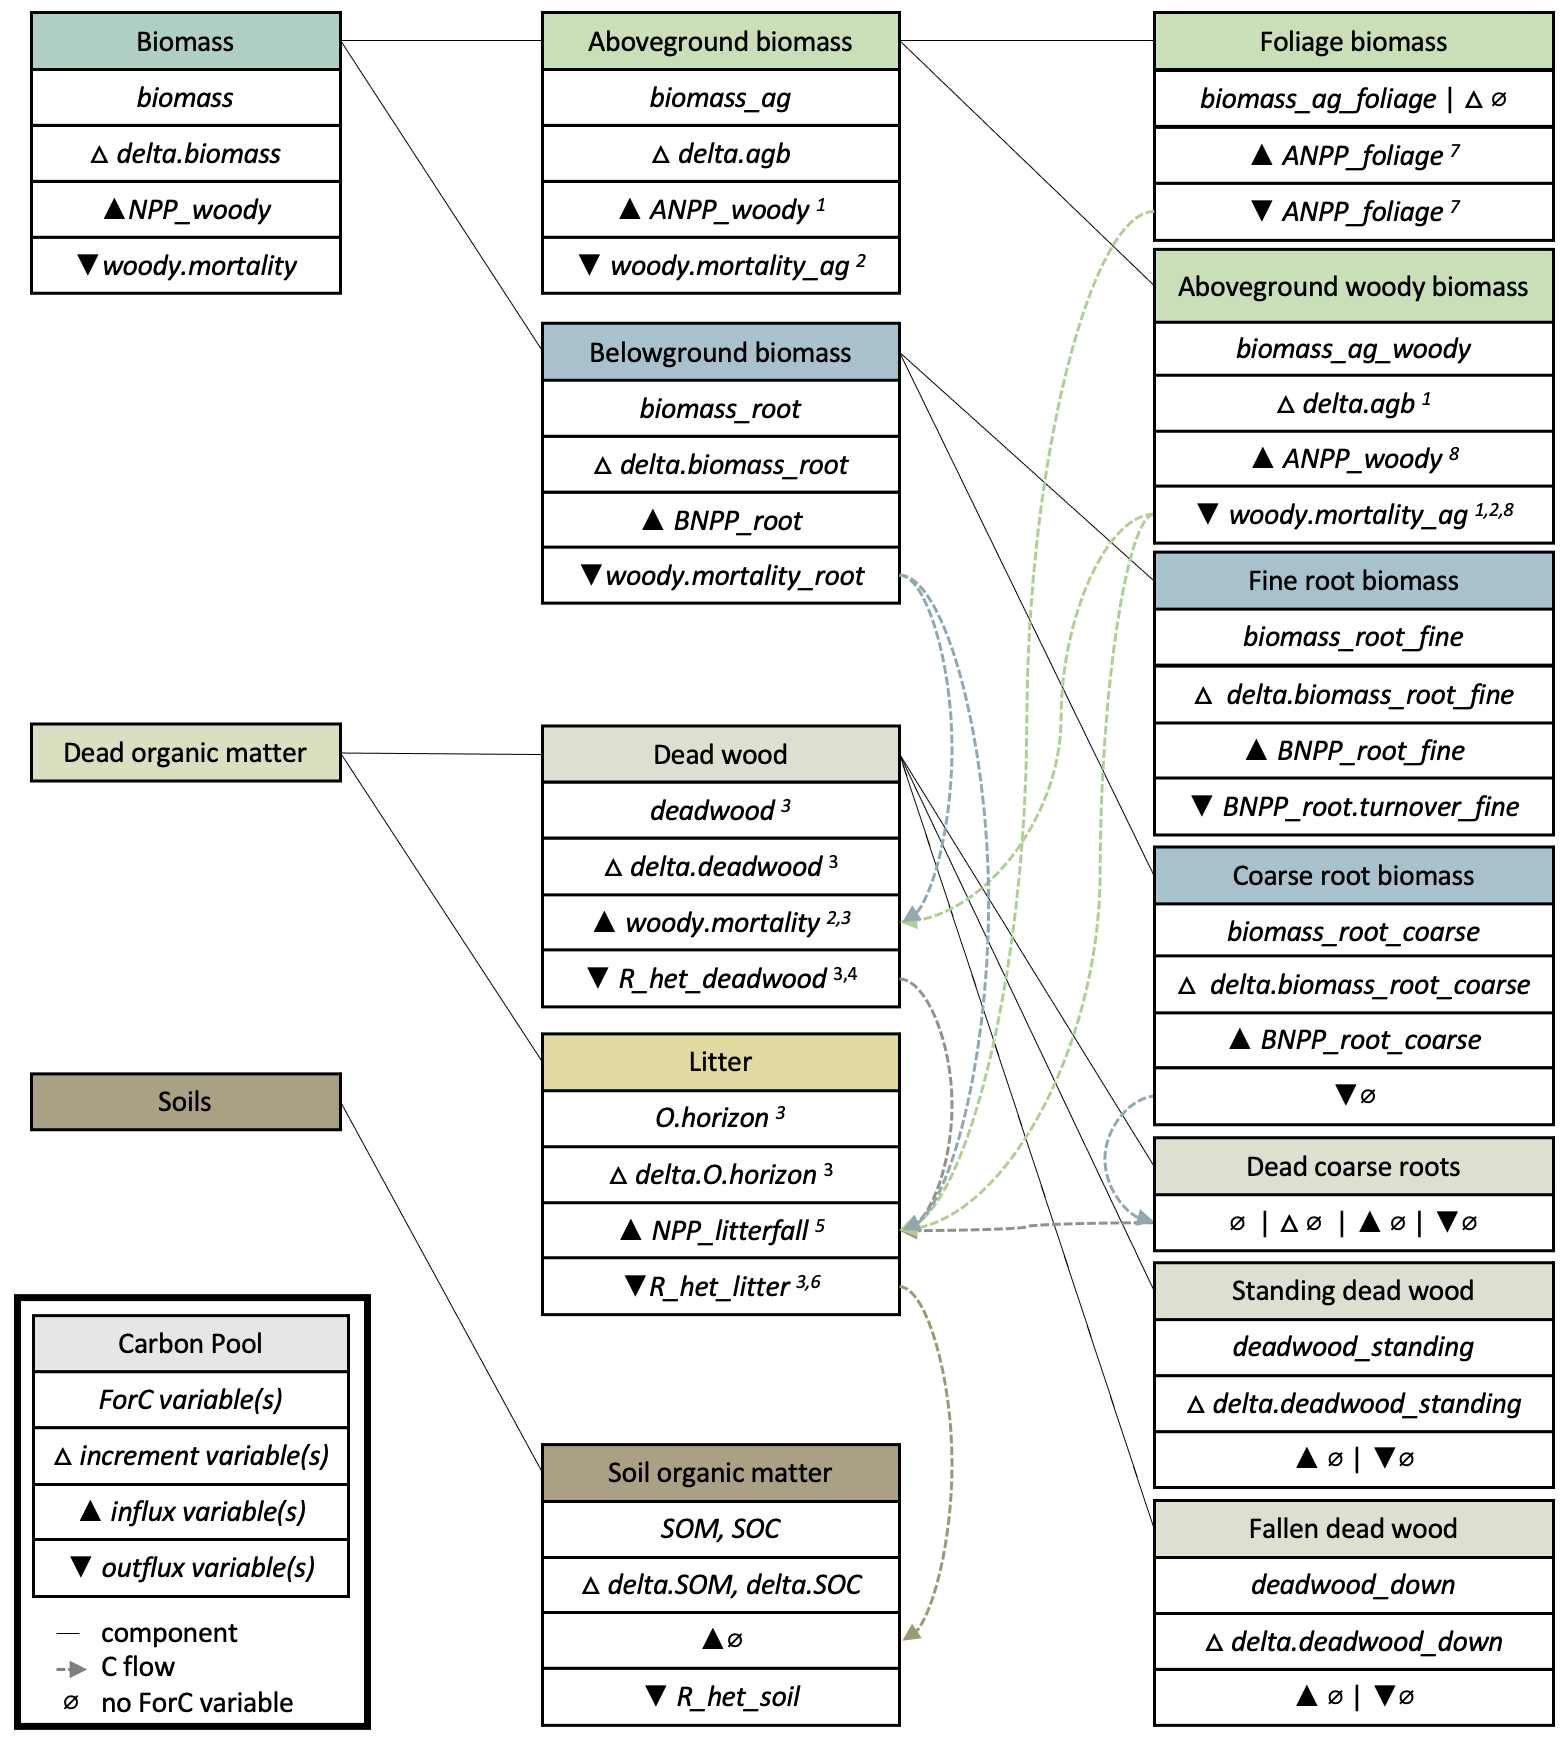
\includegraphics[width=14cm]{figures_tables/C_variable_mapping} \caption{\textbf{Schematic illustrating the carbon pools defined under IPCC Guidelines for national greenhouse gas inventories; corresponding ForC variables, and relationships among them.} For each C pool, we show ForC variables corresponding to the stock, stock change (net annual increment), gain (influx), and loss. Most, but not all, EFDB-relevant ForC variables are shown here. Correspondence of ForC variables to IPCC criteria often depends upon measurement protocols (e.g., minimum stem diameter censused). Additional caveats are as follows: (a,b) branch fall and mortality of stems below the minimum stem diameter censused, which are necessary for a full accounting of dead organic matter production but typically assumed negligible for calculations of biomass change, are excluded by common measurement practice (a) or ForC variable definition (b); (c) assumes that leaf production equals leaf fall, or that changes in foliage biomass are negligble; (d,e) belowground components excluded by common measurement practice (d) or ForC variable definition (e); (f) excludes movement of dead wood into litter through breakage or size reduction; (g) measurements often limited to litter horizon (OL) and may exclude larger branches and stems classified as litter and/or the more decomposed layers of the O horizon. **This variable is techically EFDB-relevant but not selected for submission because their is no corresponding influx variable.}\label{fig:fig_variable_mapping}
\end{figure}

\subsection{Quality control measures}

Prior to releasing ForC v4.0, we executed several quality control
measures. First, we implemented a system of continuous integration using
GitHub Actions \citep[\emph{sensu}][]{kim_implementing_2022} to run some
automatic checks any time the master data files are updated, including
outlier tests and checks for completeness and naming consistency of
records across data files. Second, to improve information on geographic
coordinates, we created a field to record coordinate precision (Appendix
A), and flagged and reviewed records with suspected low precision.
Third, to identify erroneous climate data, we compared ForC climate
values to those extracted from WorldClim version 2.1
\citep{vandepol_identifying_2016, bailey_climwin_2016} based on site
coordinates. Records deviating from WorldClim values by more
variable-specific thresholds (\textgreater5°C for mean annual
temperature, \textgreater7.5°C for mean temperatures of the warmest and
coldest months, or \textgreater1 for log(mean annual precipitation in
mm)) were flagged as requiring review prior to use in analysis or
submission to EFDB.

Because ForC v4.0 contained known duplicate records, we used R scripts
to identify likely duplicates, as detailed in
\citet{anderson-teixeira_carbon_2021}. Henceforth, we refer to the set
of records with likely duplicates removed as ``independent records''.
All records sent to EFDB were ensured to be independent and original
through manual review, as detailed below.

\subsection{Manual review of records to be sent to EFDB}

EFDB data submissions required information that was not recorded in
previous versions of ForC, but for which new fields were created for
EFDB compatibility (Appendix A). It was therefore necessary to return to
original publications to retrieve relevant information, including (1)
estimates in original units, (2) confidence intervals (when not already
in ForC), (3) whether records of interest were presented in tables or
text or digitized from figures (EFDB will not accept digitized data),
(4) whether records of interest were presented directly, as opposed to
having been calculated from related variables (for example, if a study
presents aboveground biomass and root biomass but not total biomass,
EFDB would not accept the sum of these as a valid record of total
biomass) We also checked that existing ForC records were complete and
correct.

Manual review of records was the limiting step for data submission to
EFDB. We prioritized review of (1) records from the Forest Global Earth
Observatory
\citep[ForestGEO,][]{anderson-teixeira_ctfsforestgeo_2015, davies_forestgeo_2021},
(2) studies with confidence intervals recorded in ForC (because
uncertainty estimates are important to the IPCC), (3) original
publications containing large numbers of EFDB-relevant records, and (4)
records from tropical regions. The latter criteria was motivated by the
fact that although tropical forest is the single most important biome
for climate change mitigation \citep{refs}, ground-based data on
tropical forest C cycling tends to be more scarce due to a variety of
challenges \citep{refs, delima_making_2022}, and tropical countries are
more likely to apply Tier 1 methodology that bases forest C budgets on
internationally defined IPCC default values
\citep{romijn_assessing_2015}.

\subsection{Addition of new records}

In addition to reviewing existing records, we added a total of 329 new
records to ForC. These included 104 records from two studies
\citep{piponiot_distribution_2022, lutz_largediameter_2021} that were
not previously included in ForC. In addition, we created new records for
225 EFDB-relevant estimates presented in the original publication that
were not yet present in ForC.

\section{Submission of ForC data to EFDB}

To submit complete, reviewed ForC records into EFDB, we created R
scripts to restructure ForC records and populate EFDB's bulk import form
(``EFDB bulk import.xlsx''). Criteria for data submission were that (1)
records had been checked against the original study and determined to be
complete and correct, and as originally presented, (2) the original
study presented values in tables or text, as opposed to the values
having been digitized from graphs or calculated based on related
variables, and (3) the records had not previously been submitted to
EFDB. Once converted into EFDB format, the records were reviewed and
then sent to the IPCC's Technical Support Unit for submission to EFDB.
Complete records needed to be reviewed by the EFDB editorial board and
then posted in the database -- a process that lags behind submission of
records and had not yet been completed for all records sent as of June
09, 2023.

\subsection{Mapping ForC to EFDB}

The mapping of ForC fields into EFDB fields is summarized in Appendix B.
For the majority of fields, contents of the field in ForC was copied
directly into an EFDB field, either as the only contents of that field
or as part of a composite record. For example, ten ForC fields
describing site location, climate, and edaphic properties all mapped
into the EFDB field \emph{Region/Regional conditions} (Appendix B). In
cases where original studies did not present 95\% confidence intervals
(required by IPCC when available) but did present information required
to calculate these (standard error or n and standard deviation), we
calculated the 95\% confidence intervals and populated the EFDB field
with this information (noting the calculation in the EFDB field
\emph{Comments from Data Provider}). For some fields, simple conditional
logic was used to populate EFDB fields based on ForC records. For
example, for stock variables presented in the original publication in
units of dry organic matter mass (as opposed to C), several greenhouse
gasses (CO\textsubscript{2}, CO, CH\textsubscript{4}, NO,
NO\textsubscript{2}, N\textsubscript{2}O) were entered in the EFDB field
indicating the greenhouse gases to which the record could be pertinent
(\emph{Gases} field) because these values could be used in calculations
of greenhouse gas emissions from biomass burning \citep{ipcc_2006_2006};
otherwise, the only pertinent greenhouse gas would be
CO\textsubscript{2}. There were two cases in which more complex mapping
was required: (1) mapping of C cycle variables (section 4.1.1) and (2)
land classification (section 4.1.2).

\subsubsection{Carbon cycle variables}

With input from the IPCC's Technical Support Unit, we reviewed the list
of ForC variables to identify those that were relevant to EFDB and to
appropriately map them into EFDB (Fig. 1). For each C pool (Table 1), we
identified variables representing organic matter or C stocks, net annual
increments, influxes (a.k.a. ``gross annual increments'' by IPCC), and
outfluxes. As described in section 3.2, we also defined 15 new
EFDB-relevant variables that were not previously represented in ForC. It
is important to note that the correspondence of ForC variables to IPCC
criteria often depends upon measurement protocols (``important sources
of estimate variation'' in Table 1). For example, ForC records of
biomass and dead wood vary in the minimum stem diameter censused, such
that some records would match the IPCC criteria whereas others would
not. Information on minimum diameters censused and other important
sources of methodological variation are recorded as covariates in ForC
and mapped into the EFDB field \emph{Other Properties} (Appendix B).
Details on the mapping of ForC variables to EFDB -- including associated
covariates, IPCC pools (Table 1) and relevant equations
\citep{ipcc_2006_2006} -- are documented in the file
ForC\_variables\_mapping.csv in the GitHub repository associated with
this publication IPCC-EFDB-integration repository in ForC-db
organization (\url{https://github.com/forc-db/IPCC-EFDB-integration}).

\subsubsection{Land classification}

Determination of the IPCC land-use category (i.e., Forest Land,
Grassland, Wetlands, Cropland, Settlements, or Other Land; section 2.2)
was made based on the categorical ForC field \emph{dominant.life.form},
sometimes drawing upon stand age. Records with ``woody''
\emph{dominant.life.form} were classified as Forest Land. Those with
\emph{dominant.life.form} of ``woody+grass'', which in ForC is
indicative of anything from a shrub-encroached grassland to a
tree-dominated savanna, were given dual classification of Forest Land
and Grassland. This dual classification indicates that records may be
relevant to either category depending on the definition of forest
applied (varies by country). For (rare) cases where
\emph{dominant.life.form} was grass and stand age was greater than zero,
indicative of early successional vegetation, we assigned a
classification of Forest Land, consistent with the IPCC definition that
Forest Land includes land expected to succeed to forest. Cases where
\emph{dominant.life.form} was grass or crop and stand age was zero were
indicative of a control for studies of forest regrowth following
agricultural abandonment, and were classified as Grassland and Cropland,
respectively.

Classification into sub-categories was dependent upon stand age and site
history (section 2.2). For Forest Land ≥ 20 years old or of unknown
(relatively mature) age, or Forest Land \textless{} 20 years old that
was forest prior to a stand-clearing disturbance, the past land-use
category was Forest Land, making the sub-category ``Forest Land
Remaining Forest land''. For forests \textless20 years old with history
including cultivation/ tillage or grazing, past land-use categories were
Cropland and Grassland, respectively, making land-use subcategories were
``Cropland converted to Forest Land'' and ``Grassland converted to
Forest Land'', respectively. For forests \textless20 years old with
unspecified previous agricultural use, we assigned the sub-category
``Land Converted to Forest land''. Forests \textless20 years old with
unknown land use prior to the study date were simply classified as
``Forest Land''. The same logic was applied for savannas, but including
both Forest Land and Grassland as potentially relevant categories.

Given the lack of public information needed to determine whether lands
are classified as managed
\citep{ogle_delineating_2018, deng_comparing_2021}, and because the
IPCC's definition of managed land is more expansive than is commonly
applied in the scientific literature and hence in ForC, we did not
include any classification of land management status from ForC in the
records submitted to EFDB. However, we did provide auxiliary information
that should be useful in making this determination, including
geographical location and notable disturbance events.

\section{Results}

\subsection{ForC v4.0 contents}

As of June 09, 2023, ForC (v4.0) contained 32693 independent records
(39848 total), 19316 of which were for the 42 variables relevant to EFDB
(Fig. 1). These records were distributed across all forested continents
and ecozones, albeit unevenly (Fig. 2). The largest number of records
came from Asia, followed by North America, South America, and Europe,
with relatively few records from Africa, Australia, and Oceania (Fig.
3c). Categorized by FAO ecozone, the greatest numbers of records came
from subtropical humid forests, temperate mountain systems, and tropical
rain forests, each with \textgreater2,000 independent records (Fig. 3b).
Boreal coniferous forests, temperate continental forests, subtropical
mountain systems, and tropical moist deciduous forests had
\textgreater1,000 independent records each, while other ecozones all had
\textless1,000 records. The most widely represented forest type was
needleleaf evergreen, followed by broadleaf deciduous and broadleaf
evergreen (Fig. 3a). In terms of stand age, the most represented age
class was 20-100 years, followed by \textless20 years and then
\textgreater100 years (Fig. 3d).

\begin{figure}
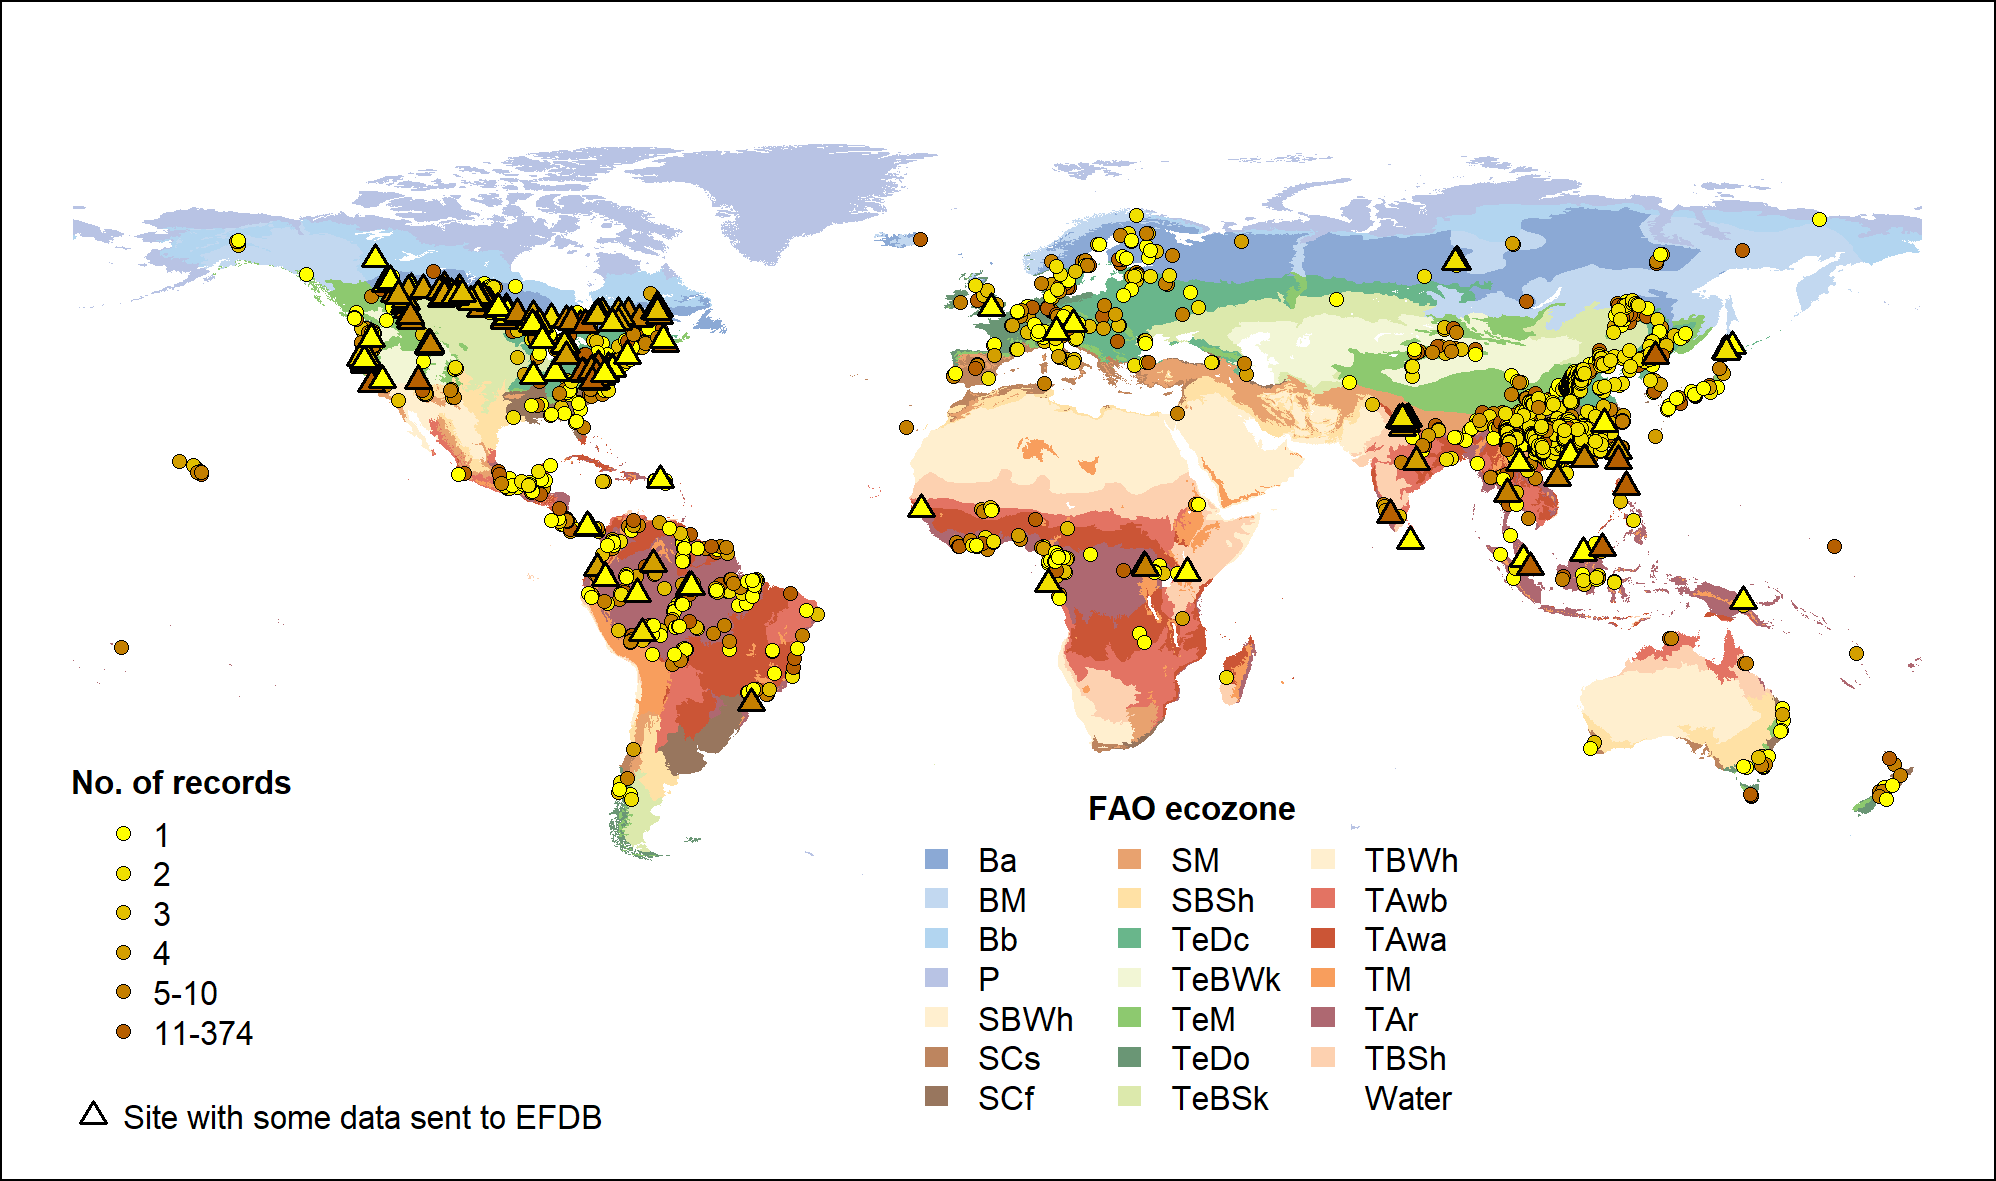
\includegraphics[width=15cm]{figures_tables/World_Map_of_sites_with_FAO_and_IPCC_data_sent} \caption{\textbf{Map of sites in ForC shaded by number of independent records relevant to (circles) and submitted to (triangles) EFDB.} Symbols are colored according to the number of records at each site. Underlying map shows FAO ecozones, which are coded as follows: Ba-Boreal coniferous forest, Bb-Boreal tundra woodland, BM-Boreal mountain systems, P-Polar, SBSh-Subtropical steppe, SBWh-Subtropical desert, SCf-Subtropical humid forest, SCs-Subtropical dry forest, SM-Subtropical mountain systems, TAr-Tropical rain forest,  TAwa-Tropical moist deciduous forest, TAwb-Tropical dry forest, TBSh-Tropical shrubland, TBWh-Tropical desert, TeBSk-Temperate steppe, TeBWk-Temperate desert, TeDc-Temperate continental forest, TeDo-Temperate oceanic forest, TeM-Temperate mountain systems, TM-Tropical mountain systems.}\label{fig:fig_map}
\end{figure}

\newpage
\begin{figure}
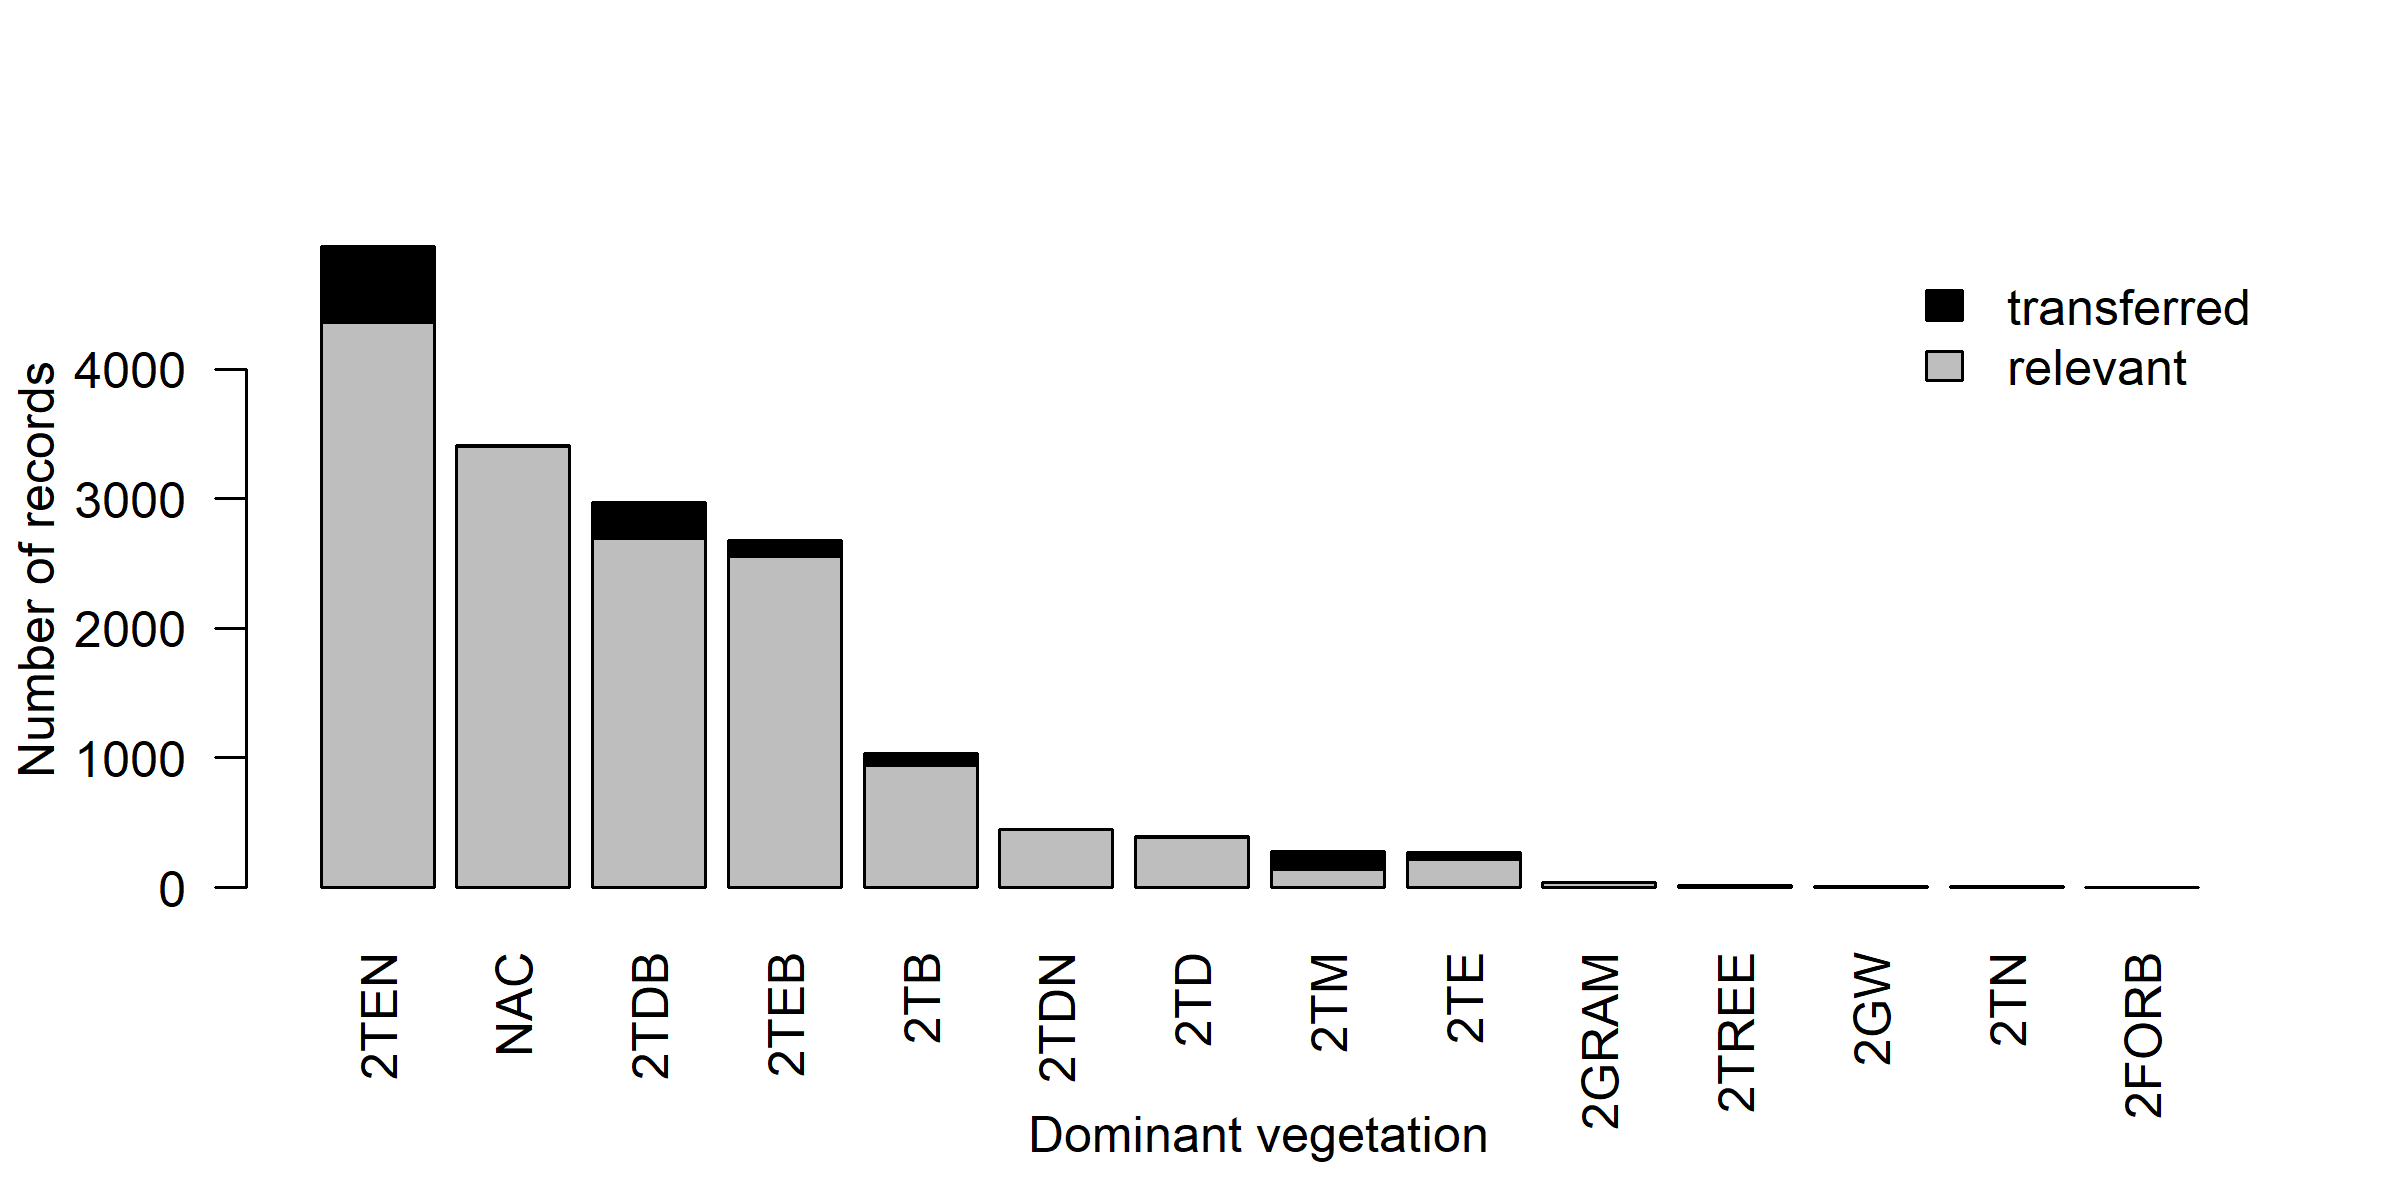
\includegraphics[width=15cm]{figures_tables/Histogram_n_Relevant_and_Transferred_Records} \caption{\textbf{Histograms of number of independent records in ForC relevant to (grey) and submitted to (black) EFDB, organized by (a) dominant vegetation type, (b) FAO ecozone, (c) continent, and (d) stand age.} For dominant vegetation (a), 'Other' includes deciduous needleleaf, mixed broadleaf- needleleaf, non-woody vegetation (e.g., early successional), and incompletely classified or mixed forest types. For FAO ecozones (b), codes are as listed in the caption of Figure 2.}\label{fig:fig_histograms}
\end{figure}

ForC contained records for 29 of the 42 variables (or closely-related
variable groups) relevant to EFDB (Table 2, Fig. 1). The records were
very unevenly distributed across variables. The variable with most
records was aboveground biomass, representing 42\% of all independent
records relevant to EFDB, and aboveground biomass components (woody
biomass or foliage) representing an additional 5\%. A total of 27\% of
relevant records were for root biomass (including fine and coarse root
components), while 4\% described total biomass. The non-living pools
were less represented, with 4\% of relevant were for dead wood
(including standing and fallen components), 0.4\% for litter, 0.3\% for
total ecosystem C excluding soils, and 2.1\% for soil carbon.

Increment and flux variables were poorly represented (Table 2). The
increment variable with most records was the aboveground biomass
increment, representing 0.8\% of all independent records relevant to
EFDB. The only other relevant increment variable with any records was
the O horizon (litter) increment, with just 4 records. Relevant flux
variable records (n=2751) together constituted 14\% of ForC's
independent records relevant to EFDB.

\newpage
\begingroup\fontsize{8}{10}\selectfont

\begin{longtable}[t]{l|l|l|l|l}
\caption{\label{tab:table_variables}\textbf{Numbers of records of ForC variables (or closely related variable groups) relevant to, and sent to, EFDB.}}\\
\hline
\textbf{variable} & \textbf{n in ForC} & \textbf{n independent records in ForC} & \textbf{n reviewed} & \textbf{n submitted to EFDB}\\
\hline
\endfirsthead
\caption[]{\textbf{Numbers of records of ForC variables (or closely related variable groups) relevant to, and sent to, EFDB.} \textit{(continued)}}\\
\hline
\textbf{variable} & \textbf{n in ForC} & \textbf{n independent records in ForC} & \textbf{n reviewed} & \textbf{n submitted to EFDB}\\
\hline
\endhead
\textbf{Biomass} & \textbf{} & \textbf{} & \textbf{} & \textbf{}\\
\hline
biomass & 1094 & 850 & 95 & 50\\
\hline
delta.biomass & 0 & 0 & 0 & 0\\
\hline
NPP\_woody & 136 & 93 & 0 & 0\\
\hline
woody.mortality & 0 & 0 & 0 & 0\\
\hline
\textbf{Aboveground biomass} & \textbf{} & \textbf{} & \textbf{} & \textbf{}\\
\hline
biomass\_ag & 9449 & 8148 & 1357 & 764\\
\hline
biomass\_ag\_woody & 460 & 366 & 10 & 10\\
\hline
biomass\_ag\_foliage & 601 & 520 & 73 & 45\\
\hline
delta.agb & 166 & 150 & 145 & 123\\
\hline
ANPP\_woody & 299 & 242 & 0 & 0\\
\hline
ANPP\_woody\_stem & 949 & 622 & 60 & 61\\
\hline
ANPP\_woody\_branch & 243 & 200 & 4 & 4\\
\hline
woody.mortality\_ag & 112 & 75 & 47 & 50\\
\hline
stem\_pC & 9 & 0 & 0 & 0\\
\hline
\textbf{Belowground biomass} & \textbf{} & \textbf{} & \textbf{} & \textbf{}\\
\hline
biomass\_root & 4629 & 4185 & 125 & 57\\
\hline
biomass\_root\_fine & 930 & 595 & 18 & 18\\
\hline
biomass\_root\_coarse & 599 & 413 & 12 & 7\\
\hline
delta.biomass\_root & 0 & 0 & 0 & 0\\
\hline
delta.biomass\_root\_coarse & 0 & 0 & 0 & 0\\
\hline
delta.biomass\_root\_fine & 0 & 0 & 0 & 0\\
\hline
woody.mortality\_root & 0 & 0 & 0 & 0\\
\hline
BNPP\_root & 577 & 416 & 0 & 0\\
\hline
BNPP\_root\_fine & 488 & 331 & 0 & 0\\
\hline
BNPP\_root.turnover\_fine & 91 & 56 & 0 & 0\\
\hline
BNPP\_root\_coarse & 329 & 250 & 0 & 0\\
\hline
\textbf{Dead wood} & \textbf{} & \textbf{} & \textbf{} & \textbf{}\\
\hline
deadwood & 438 & 304 & 104 & 70\\
\hline
deadwood\_standing & 153 & 121 & 18 & 17\\
\hline
deadwood\_down & 425 & 369 & 52 & 28\\
\hline
delta.deadwood & 0 & 0 & 0 & 0\\
\hline
delta.deadwood\_standing & 0 & 0 & 0 & 0\\
\hline
delta.deadwood\_down & 0 & 0 & 0 & 0\\
\hline
R\_het\_deadwood & 0 & 0 & 0 & 0\\
\hline
\textbf{Litter} & \textbf{} & \textbf{} & \textbf{} & \textbf{}\\
\hline
O.horizon & 45 & 45 & 45 & 40\\
\hline
delta.O.horizon & 4 & 4 & 4 & 4\\
\hline
litter & 30 & 30 & 23 & 23\\
\hline
delta.litter & 0 & 0 & 0 & 0\\
\hline
ANPP\_litterfall & 294 & 253 & 11 & 11\\
\hline
NPP\_litter & 94 & 70 & 0 & 0\\
\hline
R\_het\_litter & 167 & 143 & 0 & 0\\
\hline
\textbf{Total Ecosystem C (excl. soils)} & \textbf{} & \textbf{} & \textbf{} & \textbf{}\\
\hline
total.ecosystem\_2 & 64 & 64 & 0 & 0\\
\hline
delta.total.ecosystem\_2 & 0 & 0 & 0 & 0\\
\hline
\textbf{Soil organic matter} & \textbf{} & \textbf{} & \textbf{} & \textbf{}\\
\hline
SOM / SOC & 693 & 401 & 89 & 56\\
\hline
delta.SOM / delta.SOC & 0 & 0 & 0 & 0\\
\hline
\textbf{TOTAL} & \textbf{23568} & \textbf{19316} & \textbf{2292} & \textbf{1438}\\
\hline
\end{longtable}
\endgroup{}

\subsection{Data submissions to EFDB}

As of June 09, 2023, we had reviewed or added 2292 EFDB-relevant
records, 1438 records of which were submitted to EFDB, and 376 of which
have been reviewed, accepted, and posted (Figs. 2-3, Table 2). The 37\%
attenuation between records reviewed and those sent to EFDB was
attributable to the presence of digitized records and records where a
variable's value had been calculated as the sum or difference of related
variables rather than presented directly in the text. The discrepancy
between the number of records sent and that posted to EFDB is primarily
attributable to the time required for the IPCC to review the records,
and it is not expected that many -- if any -- records will be rejected.

The ForC records submitted to EFDB were broadly distributed across
Earth's forests (Fig. 2). However, the density of these records was very
unevenly distributed across continents, biomes, and forest types and was
not proportional to the numbers of relevant records in ForC (Fig. 3).
Rather, the largest number of records came from North America, followed
by Asia, South America, and Africa (Fig. 3c), with the most represented
FAO ecozones being boreal coniferous forest, temperate continental
forest, and temperate mountain systems, followed by tropical rain
forests and moist deciduous forests (Fig. 3b). In terms of dominant
vegetation, by far the most records came from needleleaf evergreen
forests, followed by broadleaf deciduous and broadleaf evergreen (Fig.
3b). The largest records came from mature forests (\textgreater100
years), followed by young and intermediate-aged stands (Fig. 3d).

In terms of variables, records were submitted for 19 variables (or
closely-related variable groups), including variables from each C pool
(Table 2). The majority (82\%) of records sent were for C stocks,
including 3\% for total biomass, 53\% for aboveground biomass, 4\% for
components of aboveground biomass (wood or foliage), 4\% for root
biomass, 2\% for components of root biomass (coarse or fine roots), 5\%
for dead wood, 3\% for components of dead wood (standing or fallen), 4\%
for litter (entire O horizon or OL layer component), and 4\% for SOM/
SOC. Increment records totaled 9\% of records sent, virtually all for
aboveground biomass (excepting 4 records for delta.O.horizon). The
remaining 9\% of records sent described fluxes, all of which were either
inputs or outputs to the aboveground biomass pool, a subset of which
also described inputs to the dead wood or litter pool (Table 2, Fig. 1).

\section{Recommendations}

Based on our experience contributing forest C data to EFDB via ForC, we
make several recommendations as to how scientists can improve forest C
records in EFDB through database work (section 6.1), new data collection
and analysis (section 6.2), and reporting (section 6.3).

\subsection{Database needs}

There is vast potential to expand forest C data in EFDB by completing
the process of reviewing and submitting data that are already in ForC
(Figs. 2-3). So far, only \textasciitilde7\% of the EFDB-relevant data
in ForC have been submitted to EFDB. Although this process requires
manual review of records, the submission of new records to EFDB is
hugely facilitated by the fact that most pertinent information for each
record is already entered in ForC and can be easily prepared for
submission to EFDB using the system developed here. Future efforts to
review studies for submission should optimize for representation across
geographic regions, forest types, and variables, giving priority to
those from currently under-represented regions and forest types (Figs.
2-3, Table 2), to records from countries relying on existing data for
their greenhouse gas inventories (Tier 1 or 2 methodology), to the
variables most needed by EFDB users, and to the more contemporary
records.

In addition to the large potential to expand EFDB using records already
in ForC, there are innumerous published EFDB-relevant forest C data that
are not currently included in ForC, with more being published on a
nearly daily basis. Coverage of particular variables or regions could be
vastly improved through systematic review of the literature. Indeed,
recent efforts have compiled large databases of relevant data from
monoculture plantation forests \citep{bukoski_rates_2022}, \ldots{}
\emph{others? (SUSAN)}. Beyond expanding collections of relevant forest
C records, such reviews are valuable for assessing the availability of
published records and identifying variables and regions that require
additional data collection and analysis.

\subsection{Data collection and analysis needs}

New data collection and analysis is needed to fill notable knowledge
gaps. While aboveground biomass stocks in particular have received --
and continue to receive -- by far the most research attention
\citep[Table
2,][]{anderson-teixeira_carbon_2021, dubayah_global_2020, quegan_european_2019, nisar_nasaisro_2018},
production of an accurate global map of forest C stocks remains an
ongoing challenge \citep{araza_decade_2023}. Other pools and variables
remain very poorly quantified \citep[Table
2,][]{anderson-teixeira_carbon_2021}, introducing substantive
uncertainties into global forest C budgets
\citep{pan_large_2011, harris_global_2021}. Furthermore, data
distribution is uneven across forest types and geographical regions
(Figs. 2-3). For instance, data on C cycling of tropical forests --
particularly in Africa -- remains relatively sparse, in large part due
to substantial barriers to data collection and distribution
\citep{delima_making_2022}. Significant investment in research and
researchers focused on ground-based measurement of forest C in such
regions will be important to filling knowledge gaps in forest C cycling
\citep{delima_making_2022, araza_decade_2023, labrière_forest_2023}.

Several EFDB-relevant variables have not been calculated and presented
as frequently as would be possible given existing forest census data and
minimal extra research effort. For example, aboveground woody mortality
(\emph{woody.mortality\_ag}) and aboveground biomass increment
(\emph{delta.agb}) can be calculated from the same census data as
aboveground woody productivity (\emph{ANPP\_woody}), yet the latter has
received far more research attention, and correspondingly has far more
records in ForC \citetext{\citealp[Table
2,][]{anderson-teixeira_carbon_2021}; \citealp[but
see][]{piponiot_distribution_2022}}. Similarly, live coarse root
biomass, total biomass, and changes in both of these pools could in
theory be estimated in parallel with aboveground biomass, with the
greatest barrier being that allometric models for estimating root
biomass are not as reliable or easily available as are those for
aboveground biomass
\citep{chave_improved_2014, rejou-mechain_biomass_2017, gonzalez-akre_allodb_2022}.
However, while equations for estimating root (and thereby total) biomass
require improvement, they do exist for many forest types
\citep[e.g.,][]{brassard_coarse_2011, chojnacky_updated_2014, waring_overlooking_2017}.
In addition, standing dead trees are captured in most forest censuses
and could be used to estimate standing dead wood, although additional
data on breakage would be needed for accurate estimates. We recommend
that, when possible, researchers calculate and report these variables,
following the reporting guidelines specified in section 6.3.

Filling knowledge gaps in other EFDB-relevant variables will require
more effort, but this effort is warranted given their importance for
estimating forest C stock chnages. Although aboveground biomass is the
most studied variable considered here (Table 2) and is the target of
satellite missions
\citep{dubayah_global_2020, quegan_european_2019, nisar_nasaisro_2018},
significant ground-based research effort is required to create accurate
global maps of forest biomass and changes therein
\citep{duncanson_importance_2019, labrière_forest_2023}. Given
observations of increasing tree mortality in some forested regions
\citep{mcdowell_pervasive_2020}, better characterization of forest dead
wood will be critical. Additionally, C stocks in forest organic horizons
and soils can be quite substantial and highly uncertain in many parts of
the world \citep{tifafi_large_2018}. Significant investment in
ground-based forest research will be critical to filling these gaps.

\subsection{Data reporting needs}

We recommend that, in order to make research valuable to estimate C
stock changes according to methods provided in the IPCC guidelines,
researchers calculate and report results according to IPCC good practice
(Table 3). It is particularly noteworthy that simple decisions on the
presentation of results will determine whether the records meet the
criteria for inclusion in EFDB. Some examples are as follows: (1)
presenting data only in a figure makes them ineligible for inclusion in
EFDB, whereas presentation in a table or supplementary data file allows
inclusion while supporting FAIR
(http://dx.doi.org/10.1038/d41586-019-01720-7) goals; (2) direct
presentation of all relevant variables allows inclusion, whereas
presenting only components of variables of interest (e.g., parsing
litter into fine woody debris, OL, OF, and OH layers) or requiring
simple mathematical operations to obtain a variable of interest (e.g.,
\emph{delta.agb} = \emph{ANPP\_woody} - \emph{woody.mortality.agb})
disqualifies records from inclusion; (3) matching IPCC-defined
thresholds for defining C pools (Table 1), which may vary by country,
can make the data far more relevant estimating forest C stock changes
according to IPCC guidelines (e.g., using a 10 cm cutoff between dead
wood and litter, presenting soil C to a depth of 30 cm). It should also
be emphasized that reporting of 95\% confidence intervals (or other
metrics of error), when applicable, is highly desirable and makes the
data more relevant to IPCC.

\begin{table}

\caption{\label{tab:table_recommendations}\textbf{Recommended best practices for reporting forest C estimates of value to national greenhouse gas inventories under IPCC guidance.}}
\centering
\fontsize{10}{12}\selectfont
\begin{tabu} to \linewidth {>{\raggedright}X>{\raggedright}X>{\raggedright}X}
\hline
\textbf{criteria} & \textbf{recommendation} & \textbf{rationale}\\
\hline
variables to include & When possible, calculate and present all relevant variables that can be readily estimated based on available data. & Estimates of relevant variables are not always calcualted.\\
\hline
forest census methods & Adopt IPCC guidelines (country-specific) for minimum stem size in censues in census and reporting. Ideally, census stem down to the smallest diameter feasible. & IPCC biomass pool definition includes all living vegetation, but understory may be excluded when contribution is minor.\\
\hline
 & Census all taxa crontributing signficantly to biomass & IPCC biomass pool definition includes all living vegetation.\\
\hline
dead organic matter sampling & Adopt IPCC recommendations for minimum diameter of deadwood (country-specific, default 10 cm). & Diameter cutoff must be applied consistently by each country.\\
\hline
belowground sampling & Select and report soil sampling increments to include a cutoff at 30 cm depth (or country-specific depth). & Diameter cutoff must be applied consistently by each country.\\
\hline
reporting variables & Present each EFDB- relevant variable individually, as opposed to requiring summation of related variables. & EFDB requires that values in the database be presented in the original article, and cannot accept subsequent calculations.\\
\hline
reporting estimates & Report all relevant values in tables, text, or supplementary tables/ data files, as opposed to in figures only. & EFDB does not accept values digitized from figures.\\
\hline
reporting confidence intervals & Report 95\% confidence intervals, standard error, or standard deviation and sample size. & EFDB requires confidence invervals whenever possible.\\
\hline
\end{tabu}
\end{table}

For those compiling published records (e.g., for meta-analyses), the
data set can have added value if all information required by EFDB is
extracted from original publications. This includes -- but is not
limited to -- retaining original values as presented without
modification or rounding, noting whether data were digitized, recording
confidence intervals, and recording all required fields (as indicated in
the EFDB's bulk import template). The significant effort required to map
a database into EFDB has been accomplished here (Appendix B), and we
welcome other researchers to use the ForC template.

Once EFDB-relevant data are available in peer-reviewed publications,
they may be submitted directly to EFDB or may use the ForC - EFDB data
pipeline developed here. For individual publications, the former option
will generally be more efficient. However, data incorporated into ForC
as well as EFDB will be more broadly useful; for example, these data may
be used for basic science
\citep[e.g.,][]{banburymorgan_global_2021, anderson-teixeira_carbon_2021},
analyses of forest-based climate change mitigation potential
\citep[e.g.,][]{cook-patton_mapping_2020, goldstein_protecting_2020},
and model benchmarking \citep{fer_ecosystem_2021}.

\section{Conclusions}

The ForC database contains large numbers of records that could
potentially be useful for estimating C stock changes applying
methodological guidance provided by the IPCC. Here we have developed a
framework for submitting these records to the EFDB, thus making those
data more accessible for reporting CO\textsubscript{2} emissions and
removals from forest land consistent with good practice in the IPCC
guidelines \citep{ipcc_2006_2006, ipcc_2019_2019}. As of June 09, 2023,
we have submitted 1438 records to EFDB. Although this represents just
7\% of relevant records in ForC, it substantially increases the number
of forest land records in EFDB. The records submitted to EFDB and
present in ForC are very unevenly distributed across variables, regions,
and forest types (Figs. 2-3, Table 2), reflecting broader patterns in
allocation of research effort.

Going forward, forest researchers can make their research more useful
for forest C inventories under IPCC guidelines by calculating and
reporting results in ways that are consistent with methodologies
provided in the IPCC guidelines (Tables 1, 3). In addition, substantial
investments in research and researchers focused on ground-based
measurement of forest C will be required to fill knowledge gaps and
thereby increase the accuracy of forest CO\textsubscript{2} inventories
for forest lands under teh Paris Agreement. This challenge is heightened
by the fact that forests are changing rapidly
\citep[e.g.,][]{mcdowell_pervasive_2020}, and data collected a decade or
more in the past may no longer be relevant. This heightens the need for
an efficient system of making forest C data accessible for national
greenhouse gas inventories. We view the system developed here for
submitting ForC data to the IPCC EFDB as one important step towards that
goal.

\clearpage

\section*{Appendix A. Updates to ForC}
\addcontentsline{toc}{section}{Appendix A. Updates to ForC}

\captionsetup[table]{labelformat=empty}

Table A1: \textbf{Table of changes to ForC fields.}
\begingroup\fontsize{8}{10}\selectfont

\begin{longtabu} to \linewidth {>{\raggedright}X>{\raggedright}X>{\raggedright}X>{\raggedright}X>{\raggedright}X}
\hline
\textbf{Table} & \textbf{Column} & \textbf{Description} & \textbf{Changes} & \textbf{Motivation}\\
\hline
\endfirsthead
\multicolumn{5}{@{}l}{\textit{(continued)}}\\
\hline
\textbf{Table} & \textbf{Column} & \textbf{Description} & \textbf{Changes} & \textbf{Motivation}\\
\hline
\endhead
Sites & coordinates.precision & Precision of geographic coordinates, as reported by source or estimated from maps. & field added & allow identification of records with poor coordinate precision\\
\hline
Measurements & data.location.within.source & Location of data within the source listed in citation.ID. & field added & facilitate review, ensure traceability\\
\hline
 & sd, se, lower95\%CI, upper 95\%CI & Standard deviation, standard error, and lower and upper 95 percent confidence intvervals, respectively. & replaces `stat` and `stat.name` & cleaner format; ability to handle assymetrical 95 percent confidence intervals\\
\hline
 & mean.in.original.units, original.units & mean value and units presented in original publication & fields added & provide IPCC with original units, reduce errors/improve reproducibility\\
\hline
 & C.conversion.factor & Assumed/ measured C content of organic matter used to convert organic matter to C. & field added & track units conversion, allow back-calculation of OM if conversion factor deemed inappropriate\\
\hline
PFT & description & Definition of the pftcode at the community level. Differs from individual level in that properly describes mixed plant functional types. & field added & \\
\hline
 & description.individual & Definition of the pftcode at the individual plant level. & field name change (previously `description`) & \\
\hline
Citations & citation.citation & Full citation. Most of these records are automatically generated in R based upon DOI lookup. & field added & field required by IPCC\\
\hline
 & citation.language & Language of original publication, automatically generated based on the title and abstract, with some manual entries and corrections. & field added & field required by IPCC\\
\hline
 & citation.url & URL of original publication, generally retrieved automatically via URL lookup. & field added & field required by IPCC\\
\hline
 & citation.abstract & Abstract, generally retrieved automatically via DOI lookup. & field added & field required by IPCC\\
\hline
 & source.type & citation source type & field added & field required by IPCC\\
\hline
 & pdf.in.repository & Indicates whether pdf of original study has been retrieved and saved in ForC's reference repository & field added & housekeeping\\
\hline
 & EFDB.ready & Indicates whether data have been checked for export to EFDB. & field added & housekeeping\\
\hline
\end{longtabu}
\endgroup{}

\clearpage

\section*{Appendix B. Mapping ForC to EFDB}
\addcontentsline{toc}{section}{Appendix B. Mapping ForC to EFDB}

Table B1: \textbf{Mapping of ForC fields to EFDB.} Details documented in
the public GitHub repository associated with the project,
IPCC-EFDB-integration repository within the ForC-db organization (file
\emph{ForC-EFDB\_mapping.csv} available at
\url{https://github.com/forc-db/IPCC-EFDB-integration/blob/main/doc/ForC-EFDB_mapping/ForC-EFDB_mapping.csv}).
See footnotes at end of table (STILL NEED TO BE PROPERLY INSERTED).
\begingroup\fontsize{8}{10}\selectfont

\begin{longtabu} to \linewidth {>{\raggedright}X>{\raggedright}X>{\raggedright}X>{\raggedright}X>{\raggedright}X}
\hline
\textbf{ForC table} & \textbf{ForC field} & \textbf{EFDB field} & \textbf{Usage} & \textbf{Required}\\
\hline
\endfirsthead
\multicolumn{5}{@{}l}{\textit{(continued)}}\\
\hline
\textbf{ForC table} & \textbf{ForC field} & \textbf{EFDB field} & \textbf{Usage} & \textbf{Required}\\
\hline
\endhead
Measurements & measurement.ID & Other Properties & direct mapping & (no)\\
\hline
 & dominant.life.form & 1996 Source/Sink Categories, 2006 Source/Sink Categories & used to determine land subcategories (see defining\_land\_subcategory.md) & yes\\
\hline
 & stand.age & 1996 Source/Sink Categories, 2006 Source/Sink Categories, Parameters/ Conditions & used to determine land subcategories (see defining\_land\_subcategory.md), directly listed in Parameters/ Conditions & (yes)\\
\hline
 & dominant.veg, veg.notes, min.dbh & Parameters/ Conditions & direct mapping/ linking to dominant.veg description & no\\
\hline
 & variable.name & - & link to variable info in ForC\_variables table & yes\\
\hline
 & date / start.date, end.date & Other Properties & direct mapping & no\\
\hline
 & mean & Value & direct mapping & yes\\
\hline
 & mean.in.original.units & Value in Common Units & direct mapping & yes\\
\hline
 & original.units & Common Unit & direct mapping & yes\\
\hline
 & lower95\%CI, upper 95\%CI, se, sd and n & Lower Confidence Limit, Upper Confidence Limit & direct or calculated & (yes)\\
\hline
 & depth, covariate\_1, cov\_1.value, covariate\_2, cov\_2.value & Other Properties & direct mapping & no\\
\hline
 & allometry\_1, allometry\_2 & Comments from Data Provider & link to biomass allometry source, when provided & no\\
\hline
 & data.location.within.source & - & confirm that data weren't digitized, facilitate finding data in original publication & yes\\
\hline
 & ForC.investigator & Data Provider, Data Provider Contact & link to Data Provider, Data Provider Contact info & yes\\
\hline
Sites & site.ID, sites.sitename & Other Properties & direct mapping & (no)\\
\hline
 & lat, lon & Region/Regional conditions & direct mapping; used to extract continent, Koeppen, and FAO.ecozone & (no)\\
\hline
 & country, state, city, masl,  mat, map & Region/Regional conditions & direct mapping & no\\
\hline
 & continent, Koeppen & Region/Regional conditions & direct mapping & auto\\
\hline
 & soil.texture, sand, silt, clay, soil.classification & Parameters/ Conditions & direct mapping & no\\
\hline
 & FAO.ecozone & Parameters/ Conditions & direct mapping & auto\\
\hline
History & date, hist.cat, hist.type & 1996 Source/Sink Categories, 2006 Source/Sink Categories, Abatement/Control technologies & used to determine distmrs.type for Source/Sink Categories, generate list of events for Abatement/Control technologies & (yes)/no**\\
\hline
 & plot.area & Other Properties & direct mapping & no\\
\hline
Plots & plot.ID, plot.name & Other Properties & direct mapping & (no)\\
\hline
 & distmrs.type & 1996 Source/Sink Categories, 2006 Source/Sink Categories & used to determine land subcategories (see defining\_land\_subcategory.md) & auto\\
\hline
 & distmrs.type, distmrs.year, regrowth.type, regrowth.year & Other Properties & direct mapping & auto\\
\hline
PFT & description & Parameters/ Conditions & direct mapping & auto\\
\hline
variables & variable.type & Gases & For stocks in unit of organic matter, gases include CO2, CO, CH4, NO, NO2, N2O. For increments, fluxes, and stocks in units of C, gases includes only CO2. & auto\\
\hline
 & variable.name & C pool, Equation & link to C pool, Equation & auto\\
\hline
 & description & Description & direct mapping & auto\\
\hline
 & extended.description & Other Properties & direct mapping & auto\\
\hline
 & units & Unit (ID) & link to IPCC units & auto\\
\hline
Citations & citation.citation & Full Technical Reference & direct mapping & yes/auto\\
\hline
 & citation.language & Reference Language & direct mapping & yes/auto\\
\hline
 & citation.url & URL & direct mapping & no/auto\\
\hline
 & citation.abstract & Abstract in English & direct mapping & no/auto\\
\hline
 & source.type & Source of Data & direct mapping & yes\\
\hline
\end{longtabu}
\endgroup{}

`Required' field indicates whether the field is required by EFDB: yes =
value required; (yes) = input required, missing value acceptable if not
reported; auto = present within ForC infrasructure, and therefore will
always be exported to EFDB ; (no) = not required for EFDB, but required
for ForC and therefore will always be exported to EFDB; no = not
required, but exported to EFDB when a value is present.

** `(yes)' for most recent severe disturbance; `no' for other history
events



\codedataavailability{All code and data are openly available. The ForC
database and associated code is available via the ForC repository within
the ForC-db organization on GitHub (https://github.com/forc-db/ForC),
and the version used here (ForC v4.0) archived in Zenodo (DOI: TBD). The
data and code associated with data submission to EFDB and preparation of
this manuscript are available via the the IPCC-EFDB-integration
repository within the ForC-db organization on GitHub
(https://github.com/forc-db/IPCC-EFDB-integration).} %% use this section when having data sets and software code available



%%%%%%%%%%%%%%%%%%%%%%%%%%%%%%%%%%%%%%%%%%
%% optional

%%%%%%%%%%%%%%%%%%%%%%%%%%%%%%%%%%%%%%%%%%

%%%%%%%%%%%%%%%%%%%%%%%%%%%%%%%%%%%%%%%%%%
\authorcontribution{KAT and VH conceived and designed the project; VH
wrote the scripts for database management, data submission to EFDB, and
the analyses presented here; MW, TR, and RBM added and reviewed ForC
data, BBL and SCP contributed large databases to ForC (EFDB and GROA,
respectively); CP provided methodological expertise; KAT, VH, and MW
prepared the first draft of the manuscript; all authors reviewed the
results and approved the final version of the
manuscript.} %% optional section

%%%%%%%%%%%%%%%%%%%%%%%%%%%%%%%%%%%%%%%%%%
\competinginterests{The authors declare no competing
interests.} %% this section is mandatory even if you declare that no competing interests are present

%%%%%%%%%%%%%%%%%%%%%%%%%%%%%%%%%%%%%%%%%%

%%%%%%%%%%%%%%%%%%%%%%%%%%%%%%%%%%%%%%%%%%
\begin{acknowledgements}
We gratefully acknowledge the substantial contributions of Valentyna
Slivinska and Sandro Federici for collaboration on the conception,
design, and technical review of this project. Thank you to all
researchers who collected and published the data contained in ForC, and
to all research assistants and collaborators who have contributed to
building the database. Thank you to Avni Malhotra for helpful comments
on an earlier draft of this manuscript. Funding for this study was
provided by the Institute for Global Environmental Strategies, a Bezos
Earth Fund award to The Nature Conservancy, and a Smithsonian Working
Land and Seascapes grant.
\end{acknowledgements}

%% REFERENCES
%% DN: pre-configured to BibTeX for rticles

%% The reference list is compiled as follows:
%%
%% \begin{thebibliography}{}
%%
%% \bibitem[AUTHOR(YEAR)]{LABEL1}
%% REFERENCE 1
%%
%% \bibitem[AUTHOR(YEAR)]{LABEL2}
%% REFERENCE 2
%%
%% \end{thebibliography}

%% Since the Copernicus LaTeX package includes the BibTeX style file copernicus.bst,
%% authors experienced with BibTeX only have to include the following two lines:
%%
\bibliographystyle{copernicus}
\bibliography{references.bib}
%%
%% URLs and DOIs can be entered in your BibTeX file as:
%%
%% URL = {http://www.xyz.org/~jones/idx_g.htm}
%% DOI = {10.5194/xyz}


%% LITERATURE CITATIONS
%%
%% command                        & example result
%% \citet{jones90}|               & Jones et al. (1990)
%% \citep{jones90}|               & (Jones et al., 1990)
%% \citep{jones90,jones93}|       & (Jones et al., 1990, 1993)
%% \citep[p.~32]{jones90}|        & (Jones et al., 1990, p.~32)
%% \citep[e.g.,][]{jones90}|      & (e.g., Jones et al., 1990)
%% \citep[e.g.,][p.~32]{jones90}| & (e.g., Jones et al., 1990, p.~32)
%% \citeauthor{jones90}|          & Jones et al.
%% \citeyear{jones90}|            & 1990


\end{document}
